%http://cs.pugetsound.edu/~jross/courses/cs240/project/requirements/
%Animation Group
\documentclass[12pt]{article}
\usepackage{graphicx}
\begin{document}




% Front Page
\begin{titlepage}
	\begin{center}
	\huge  Edith \\
	\vspace*{\fill}%
 	\huge \textsc{\textbf{Animation Team \\Requirement Specifications} }	
	\bigskip 
	\rule{130mm}{.1pt}
	\textsc{\textbf{September 25, 2013 \\ Revised: September 28, 2013} \\ }	
	\vspace*{\fill}%
	Eric Lund \\
	Kramer Canfield \\ 
	Zeke Rosenberg \\
	Calder Whiteley \\
	Jon Youmans
	\end{center}
	\end{titlepage}

% Next page

%Executive Summary
\section{\emph{Executive Summary}}
One of the components of the "Edith" system, a 2D web-based computer science teaching tool, is the Animation System module, a sub-system of Edith. The Animation System module is important because it includes the core animation frameworks and specifications of how the animations and audio will be produced. In a visually-based programming environment, this module is clearly important because it provides animations without requiring the user to have any knowledge of a scripting language or computer graphics concepts. There is only one use case for this module: provide animations and play sounds. The animations are specified by a different sub-system which delivers the instructions to the Animation System module. The Animation System processes the instructions (assuming the instructions were delivered correctly) and delivers the animations and audio to another sub-system to be displayed on the screen as desired.


%Introduction
\section{\emph{Introduction}}%Create a section for the introduction
	\subsection{Edith}
         Edith is a 2D, web-based system to help students learn to program and get excited about computer science. The system will allow students to program relationships among objects in a virtual world, in order to create animations. It will offer several useful capabilities: users will be able to create objects for their story using a graphical, drag and drop interface; specify animated behaviors for these objects using a visual programming language; add user interactions to create game-like experiences; and share their creations with others. 
	\subsection{Module}
	The Animation Module accepts a properly formatted instruction set to construct an animated scene. An animated scene consists of a canvas that can include pre-defined image sprites and pre-defined audio files provided by the Object Creator Module. The scene is installed in the final UI by the Story Creator Module. 
	\subsection{Purpose}
        The Animation Module allows the user to render animations without knowledge of a scripting language. This is possible by applying pre-defined animation sets to image sprites. The module also allows the user to include audio with their animations. The module is intended to interpret animation instructions and render an animation sequence.


% Use Cases
\section{\emph{Functional Requirements}}
	\subsection{"Use Case 1: Providing Animations and Playing Sounds"}
\begin{enumerate}
  \item Actor
  \begin{enumerate}
  		\item "Drawer": The system providing us with sprites to animate and sounds to play.
   		 \item "Taker": The system that takes and displays our canvas.
		\item Animation System: The system we are creating that handles back-end animation and final.
  \end{enumerate}
  \item Preconditions/Assumptions
  \begin{enumerate}
   		 \item Preconditions: The user has already defined which sprites will be animated and which sounds will be played.
   		 \item Assumptions: The web browser supports HTML5 and JavaScript.
  \end{enumerate}
  \item Flow of Events
  \begin{enumerate}
   		 \item "Drawer" provides drawing instructions to the Animation System. 
   		 \item The Animation System processes the instructions.
		\item The Animation System creates animations and plays sounds.
		\item The Animation System provides the animations to the "Taker."
  \end{enumerate}
  \item Alternatives
  \begin{enumerate}
    		\item The "Drawer" provides faulty drawing instructions.
    		\item The Animation System attempts and fails to process instructions.
		\item The Animation System passes the error to the "Taker."
  \end{enumerate}
  %\item  Postconditions
  %\begin{enumerate}
  % 		\item 
  %\end{enumerate}
\end{enumerate}

	

\subsection{UML}
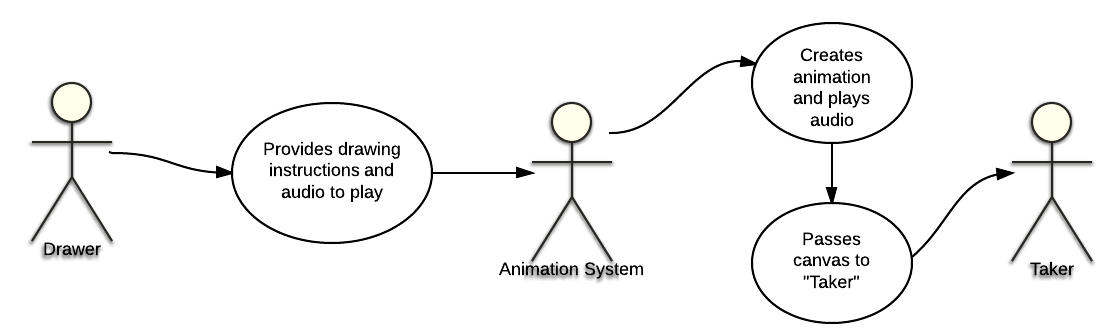
\includegraphics[scale=.4]{UML.png}
UML Diagram of Animation System Flow of Events


%Nonfunctional Requirements
\section{\emph{Nonfunctional Requirements}}

\begin{itemize}
	\item Ease-of-Use: Specific documentation of options for animation provided to the "Drawer" on animations that we can provide.
	\item Documentation: Specific documentation of instructions provided to the "Taker" on how to receive the dynamic picture frame (the canvas).
\end{itemize}

%Glossary/References
\section{\emph{Glossary/References}}
Glossary:
\begin{itemize}
	\item Canvas: The JavaScript and HTML5 "dynamic picture frame" to give to the "Taker."
	\item Sprite:  a computer graphic that may be moved on-screen and otherwise manipulated as a single entity
\end{itemize}

\noindent References: 
\begin{itemize}
	\item LaTeX WikiBook http://en.wikibooks.org/wiki/LaTeX
	\item Edith Project Description http://cs.pugetsound.edu/~jross/courses/cs240/project/edith/
	\item New Oxford American Dictionary (American English)
\end{itemize}

\end{document}
